\documentclass{article}

% Language setting
% Replace `english' with e.g. `spanish' to change the document language
\usepackage[english]{babel}

% Set page size and margins
% Replace `letterpaper' with `a4paper' for UK/EU standard size
\usepackage[letterpaper,top=2cm,bottom=2cm,left=3cm,right=3cm,marginparwidth=1.75cm]{geometry}

% Useful packages
\usepackage{amsmath}
\usepackage{graphicx}
\usepackage[colorlinks=true, allcolors=blue]{hyperref}
\usepackage{amssymb}
\usepackage{tikz}
\usetikzlibrary{positioning, arrows.meta, quotes}

\title{Linear Algebra}
\date{}

\begin{document}
\maketitle

\tableofcontents

\newpage
\section{Linear Transformation and Matrix}

\subsection{Linear Transformation (Linear Mapping)}

A function $f$ is a \textbf{Linear Mapping} if:
\begin{itemize}
    \item \textbf{Additivity}: $f(\mathbf{u}+\mathbf{v}) = f(\mathbf{u}+\mathbf{v})$.
    \item \textbf{Homogeneity}: $f(c\mathbf{u}) = c f(\mathbf{u})$
\end{itemize}

\subsection{Matrix}

Matrix $A \in \mathbb{R}^{m \times n}$ defines a \textbf{Linear Transformation} from Domain $\mathbb{R}^n$ to Codomain $\mathbb{R}^m$.
\newline
Matrix $A$ is composed of column vectors $\mathbf{a}_j$, each of which is the image of the $j$-th standard basis vector after applying the transformation $A$.
\[
    A
\]
Expanded form~\ref{eq:matrix}

\subsection{Mapping Types}

\subsubsection{Homogeneous Mapping}
A \textbf{Homogeneous Mapping} is a linear transformation.
\[
    f(\mathbf{x}) = A\mathbf{x}
\]

\subsubsection{Affine Mapping}
An \textbf{Affine Mapping} is not a linear transformation.
\[
    f(\mathbf{x}) = A\mathbf{x} + \mathbf{b}
\]


\newpage
\section{Matrix Operation}

\subsection{Inner Product}
The \textbf{Inner Product} (Dot Product) of two vectors $\mathbf{a}, \mathbf{b} \in \mathbb{R}^n$ is defined as:
\[
    \langle \mathbf{a}, \mathbf{b} \rangle = \mathbf{a}^{\mathrm{T}} \mathbf{b} = \sum_{i=1}^n a_i b_i
\]
Expanded form~\ref{eq:innerprod}.

\subsection{Norm}
The \textbf{Euclidean Norm} or $L^2$-norm of a vector $\mathbf{x} \in \mathbb{R}^n$, denoted as $\|\mathbf{x}\|$ or $\|\mathbf{x}\|_2$, is a measure of its Euclidean length.
\[
    \|\mathbf{x}\|^2 = \langle \mathbf{x}, \mathbf{x} \rangle = \mathbf{x}^{\mathrm{T}} \mathbf{x}
\]

\subsection{Frobenius Inner Product}
For matrices $A, B \in \mathbb{R}^{m \times n}$:
\[
    \langle A, B \rangle_F = \sum_{i=1}^{m} \sum_{j=1}^{n} a_{ij} b_{ij}
\]
\paragraph{Trace Formula:}
\[
    \langle A, B \rangle_F = \operatorname{tr}(A^{\mathrm{T}} B) = \operatorname{tr}(B A^{\mathrm{T}})
\]

\subsection{Frobenius Norm}
For a matrix $A \in \mathbb{R}^{m \times n}$:
\[
    \|A\|^2_F = \langle A, B \rangle_F = \sum_{i=1}^m \sum_{j=1}^n a_{ij}^2
\]

\subsection{Outer Product}
The \textbf{Outer Product} of two vectors $\mathbf{a} \in \mathbb{R}^m$ and $\mathbf{b} \in \mathbb{R}^n$ is an $m \times n$ matrix:
\[
    \mathbf{a} \otimes \mathbf{b} = \mathbf{a} \mathbf{b}^{\mathrm{T}}
\]
Expanded form~\ref{eq:outerprod}.

\subsection{Matrix and Column Vector Multiplication}
Apply Linear Transformation $A \in \mathbb{R}^{m \times n}$ to vector $\mathbf{x} \in \mathbb{R}^n$ and produce a new vector $A\mathbf{x} \in \mathbb{R}^m$.

\subsubsection{Column-wise View (Linear Combination)}
\[
    A\mathbf{x} = \sum_{j=1}^n x_j \mathbf{a}_j
\]
Expanded form~\ref{eq:matvec_col}.
\paragraph{Geometric Interpretation:} Map the standard basis vectors in the Domain $\mathbb{R}^n$ to the column vectors in the Codomain $\mathbb{R}^m$.

\subsubsection{Row-wise View (Inner Product)}
\[
    (A\mathbf{x})_i = \mathbf{a}_i^{\mathrm{T}} \mathbf{x}
\]
Expanded form~\ref{eq:matvec_row}.

\subsection{Row Vector and Matrix Multiplication}
Apply Linear Transformation $A \in \mathbb{R}^{m \times n}$ to a row vector $\mathbf{y}^{\mathrm{T}} \in \mathbb{R}^{1 \times m}$ from the left and produce a new row vector $\mathbf{y}^{\mathrm{T}} A \in \mathbb{R}^{1 \times n}$.
\[
    \mathbf{y}^{\mathrm{T}} A = \sum_{i=1}^m y_i \mathbf{a}_i^{\mathrm{T}}
\]
Expanded form~\ref{eq:rowvecmat}.
\paragraph{Geometric Interpretation:} Map the standard basis vectors in the Codomain $\mathbb{R}^m$ to the row vectors in the Domain $\mathbb{R}^n$.

\subsection{Matrix and Matrix Multiplication}
Apply transformation $B$, then apply transformation $A$.

\subsubsection{Column-wise View}
\[
    (AB)_{*j} = A\mathbf{b}_j
\]
Expanded form~\ref{eq:mul_colwise}.

\subsubsection{Inner Product View}
\[
    (AB)_{ij} = \mathbf{a}_i^{\mathrm{T}} \mathbf{b}_j
\]
Expanded form~\ref{eq:mul_inner}.

\subsubsection{Outer Product View}
\[
    AB = \sum_{k=1}^n \mathbf{a}_k \mathbf{b}_k^{\mathrm{T}}
\]
Expanded form~\ref{eq:mul_outer}.

\subsubsection{Associative Law}
\[
    (AB)C = A(BC)
\]

\subsection{Inverse}
Reverses the transformation of $A$.
\[
    A A^{-1} = A^{-1} A = I_n
\]
Calculation~\ref{subsec:gauss}.
\paragraph{Inverse of a Product Rule:}
\[
    (AB)^{-1} = B^{-1}A^{-1}
\]
\paragraph{Properties:} A square matrix $A \in \mathbb{R}^{n \times n}$ is invertible iff it has full rank, i.e., $\operatorname{rank}(A) = n$.

\subsection{Determinant}
The \textbf{determinant} of a square matrix $A \in \mathbb{R}^{n \times n}$ is denoted as:
\[
    \det(A)
\]
\paragraph{Geometric Interpretation:} The oriented volume change factor.
\paragraph{Properties:}
\begin{itemize}
    \item $A \in \mathbb{R}^{n \times n}$ has Full Rank iff $\det(A) \neq 0$.
    \item \textbf{Determinant as the product of eigenvalues}: $\det(A) = \prod_{i=1}^n \lambda_i$.
\end{itemize}
\paragraph{Calculation:}
\begin{itemize}
    \item \textbf{$2 \times 2$ Matrix:} For $A = \begin{bmatrix} a & b \\ c & d \end{bmatrix}$, $\det(A) = ad - bc$
    \item \textbf{$n \times n$ Matrix:}~\ref{subsec:cofactor}.
\end{itemize}

\subsection{Trace}
The \textbf{trace} of a square matrix $A \in \mathbb{R}^{n \times n}$ is the sum of the elements on the main diagonal:
\[
    \operatorname{tr}(A) = \sum_{i=1}^n a_{ii}
\]
\paragraph{Geometric Interpretation:} The change rate of oriented volume. Viewing the Matrix as a Vector Field, the trace is its divergence.
\paragraph{Properties:}
\begin{itemize}
    \item \textbf{Trace as the sum of eigenvalues:} $\operatorname{tr}(A) = \sum_{i=1}^n \lambda_i$
    \item \textbf{Cyclic Property:} $\operatorname{tr}(AB) = \operatorname{tr}(BA)$
\end{itemize}

\subsection{Transpose}
\[
    (A^{\mathrm{T}})_{ij} = a_{ji}
\]
\[
    \langle A\mathbf{x}, \mathbf{y} \rangle = \langle \mathbf{x}, A^{\mathrm{T}}\mathbf{y} \rangle
\]
Expanded form~\ref{eq:trans}.
\paragraph{Geometric Interpretation:} Preserves the scaling factors of $A$ but reverses the rotation/reflection directions of $A$ by swapping domain and codomain orientations.
\paragraph{Transpose Distribution Rule:}
\[
    (AB)^{\mathrm{T}} = B^{\mathrm{T}} A^{\mathrm{T}}
\]


\newpage
\section{Vecctor Spaces and Subspaces}

\subsection{Linear Independence}
A set of vectors $\{\mathbf{v}_i\}_{i=1}^n$ is \textbf{Linearly Independent} if the only solution to the equation:
\[
    \sum_{i=1}^{n} c_i \mathbf{v}_i = \mathbf{0}
\]
is the trivial solution, where all coefficients $c_i = 0$. Otherwise, the set is \textbf{Linearly Dependent}.
\paragraph{Geometric Interpretation:} Each vector in the set adds a new dimension to the space spanned by the others.

\subsection{Span}

\[
    \operatorname{span}(\{\mathbf{v}_i\}_{i=1}^{k}) = \left\{ \sum_{i=1}^{k} c_i \mathbf{v}_i : c_i \in \mathbb{R} \right\}
\]

\subsection{Column Space}
The \textbf{Column Space} (or \textbf{Range}) of a matrix $A \in \mathbb{R}^{m \times n}$ is the subspace of Codomain $\mathbb{R}^m$ spanned by the columns of $A$:
\[
    \text{Col}(A) = \{ A\mathbf{x} : \mathbf{x} \in \mathbb{R}^n \}
\]
\paragraph{Geometric Interpretation:} The subspace of the Codomain representing all directions that \textbf{can be reached} by the transformation $A$.

\subsection{Null Space}
The \textbf{Null Space} (or \textbf{Kernel}) of a matrix $A \in \mathbb{R}^{m \times n}$ is:
\[
    \ker(A) = \{ \mathbf{x} \in \mathbb{R}^n : A\mathbf{x} = \mathbf{0} \}
\]
\paragraph{Geometric Interpretation:} The subspace of the Domain containing the component of any input vector that is \textbf{discarded} by $A$.

\subsection{Row Space}
The \textbf{Row Space} of a matrix $A \in \mathbb{R}^{m \times n}$ is the subspace of Domain $\mathbb{R}^n$ spanned by the rows of $A$:
\[
    \text{Row}(A) = \{ \mathbf{y}^{\mathrm{T}} A : \mathbf{y} \in \mathbb{R}^m \}
\]
\[
    \text{Row}(A) = \text{Col}(A^{\mathrm{T}}) = \{ A^{\mathrm{T}}\mathbf{y} : \mathbf{y} \in \mathbb{R}^m \}
\]
\paragraph{Geometric Interpretation:} The subspace of the Domain containing the component of any input vector that is \textbf{preserved and transformed} by $A$.

\subsection{Left Null Space}
The \textbf{Left Null Space} (or \textbf{Cokernel}) of a matrix $A \in \mathbb{R}^{m \times n}$ is:
\[
    \operatorname{coker}(A) = \{ \mathbf{y} \in \mathbb{R}^m : \mathbf{y}^{\mathrm{T}} A = \mathbf{0}^{\mathrm{T}} \}
\]
\[
    \operatorname{coker}(A) = \ker(A^{\mathrm{T}}) = \{ \mathbf{y} \in \mathbb{R}^m : A^{\mathrm{T}} \mathbf{y} = \mathbf{0} \}
\]
\paragraph{Geometric Interpretation:} The subspace of the Codomain representing all directions that \textbf{cannot be reached} by the transformation $A$.

\subsection{Rank}
The \textbf{Rank} of a matrix $A$ is the dimension of the Column Space or Row Space of $A$.
\paragraph{Codomain:}
The Column Space is the \textbf{orthogonal complement} of the Left Null Space.
\[
    \text{Col}(A) = (\operatorname{coker}(A))^{\perp}
\]
\[
    \operatorname{rank}(A) + \dim(\operatorname{coker}(A)) = m
\]
\paragraph{Domain:}
The Row Space is the \textbf{orthogonal complement} of the Null Space.
\[
    \text{Row}(A) = (\ker(A))^{\perp}
\]
\[
    \operatorname{rank}(A) + \dim(\ker(A)) = n
\]


\newpage
\section{Special Matrix}

\subsection{Identity Matrix}
The diagonal entries are all 1, and all off-diagonal entries are 0.
\[
    (I_n)_{ij} =
    \begin{cases}
        1, & i = j \\
        0, & i \neq j
    \end{cases}
\]
Expanded form~\ref{eq:iden}.
\paragraph{Geometric Interpretation:} No transformation

\subsection{Diagonal Matrix}
The diagonal entries can be any value, and all off-diagonal entries are 0.
\[
    (D_n)_{ij} =
    \begin{cases}
        d_i, & i = j \\
        0, & i \neq j
    \end{cases}
\]
Expanded form~\ref{eq:diagm}.
\paragraph{Geometric Interpretation:} Scale the $i$-th standard basis vector by $d_i$
\paragraph{Inverse of a Diagnal Matrix:}
\[
    (D_n^{-1})_{ij} =
    \begin{cases}
        \frac{1}{d_i}, & i = j \\
        0, & i \neq j
    \end{cases}
\]
Expanded form~\ref{eq:diagminv}.

\subsection{Orthogonal Matrix (Unitary Matrix)}
All column vectors are unit vectors and orthogonal to each other.
\[
    Q^{\mathrm{T}} Q = Q Q^{\mathrm{T}} = I_n
\]
\[
    Q^{\mathrm{T}} = Q^{-1}
\]
\paragraph{Geometric Interpretation:} Rotation or reflection

\subsection{Symmetric Matrix}
\[
    A = A^{\mathrm{T}}
\]
\paragraph{Geometric Interpretation:} Scaling Transformation along orthogonal basis
\paragraph{Properties:} Eigenvectors corresponding to distinct eigenvalues are orthogonal.


\newpage
\section{Matrix Decomposision}

\subsection{Eigenvector \& Eigenvalue}

An unit \textbf{Eigenvector} $\|\mathbf{v}\| = 1$ of a Symmetric Matrix $A \in \mathbb{R}^{n \times n}$ is scaled by its corresponding \textbf{Eigenvalue} $\lambda$ when the transformation $A$ is applied.
\[
    A\mathbf{v} = \lambda \mathbf{v}
\]
\paragraph{Matrix Form:}
\[
    AV = V\Lambda
\]
where:
\begin{itemize}
    \item $V$ is a matrix whose columns are the Eigenvectors of $A$.
    \item $\Lambda$ is a diagonal matrix whose diagonal entries are the Eigenvalues $A$.
\end{itemize}
\paragraph{Calculation:}
\[
    \det(A - \lambda I) = 0
\]

\subsection{Spectral Decomposition}

Symmetric Matrix $A \in \mathbb{R}^{n \times n}$ can be decomposed as:
\[
    A = Q \Lambda Q^{\mathrm{T}}
\]
where:
\begin{itemize}
    \item $Q$ is an orthogonal matrix whose columns are a set of orthonormal Eigenvectors of $A$.
    \item $\Lambda$ is a diagonal matrix whose diagonal entries are the Eigenvalues of $A$.
\end{itemize}
\paragraph{Geometric Interpretation:}
\begin{enumerate}
    \item $Q^{\mathrm{T}}$: Rotate or reflect the basis of the vector space to the Eigenvector basis.
    \item $\Lambda$: Apply a scaling transformation along the new axes by the Eigenvalues.
    \item $Q$: Rotate or reflect the basis of the vector space back to the standard basis.
\end{enumerate}

\subsection{Eigen Decomposition (Similarity and Diagonalization)}

Square matrix $A \in \mathbb{R}^{n \times n}$ with $n$ linearly independent eigenvectors can be decomposed as:
\[
    A = P \Lambda P ^{-1}
\]
where:
\begin{itemize}
    \item $P$ is a matrix whose columns are the Eigenvectors of $A$.
    \item $\Lambda$ is a diagonal matrix whose diagonal entries are the Eigenvalues of $A$.
\end{itemize}
Matrix $A$ is \textbf{similar} to diagonal matrix $\Lambda$.
\newline
Matrix $P$ \textbf{diagonalizes} matrix $A$.
\paragraph{Geometric Interpretation:}
\begin{enumerate}
    \item $P^{-1}$: Change the basis of the vector space to the Eigenvector basis.
    \item $\Lambda$: Apply a scaling transformation along the new axes by the Eigenvalues.
    \item $P$: Change the basis of the vector space back to the standard basis.
\end{enumerate}

\subsection{Matrix Function}

For any scalar function $f$ and diagonalizable $A = P \Lambda P^{-1}$:
\[
    f(A) = P f(\Lambda) P^{-1}
\]
where $f$ applies element-wise to $\Lambda$.

\subsection{Singular Value Decomposition (SVD)}

\subsubsection{Derivation}
Assume that matrix $A \in \mathbb{R}^{m \times n}$ can be decomposed as:
\[
    A = U \Sigma V^{\mathrm{T}}
\]
where $U \in \mathbb{R}^{m \times m}$ and $V \in \mathbb{R}^{n \times n}$ are orthogonal matrices, and $\Sigma \in \mathbb{R}^{m \times n}$ is a diagonal matrix.
\[
    A^{\mathrm{T}} A = (U \Sigma V^{\mathrm{T}})^{\mathrm{T}} (U \Sigma V^{\mathrm{T}}) = V \Sigma^{\mathrm{T}} U^{\mathrm{T}} U \Sigma V^{\mathrm{T}} = V (\Sigma^{\mathrm{T}} \Sigma) V^{\mathrm{T}}
\]
\[
    AA^{\mathrm{T}} = (U \Sigma V^{\mathrm{T}})(U \Sigma V^{\mathrm{T}})^{\mathrm{T}} = U \Sigma V^{\mathrm{T}} V \Sigma^{\mathrm{T}} U^{\mathrm{T}} = U (\Sigma \Sigma^{\mathrm{T}}) U^{\mathrm{T}}
\]

\subsubsection{Singular Vector \& Singular Value}
For a matrix $A \in \mathbb{R}^{m \times n}$ with $\operatorname{rank}(A) = r$:

\begin{itemize}
    \item \textbf{Right Singular Vectors:} The columns $\mathbf{v}_i$ of $V \in \mathbb{R}^{n \times n}$ are the orthonormal eigenvectors of $A^{\mathrm{T}} A$.
    \[
        A^{\mathrm{T}} A V = V (\Sigma^{\mathrm{T}} \Sigma)
    \]
    where $\Sigma^{\mathrm{T}} \Sigma \in \mathbb{R}^{n \times n}$ is a diagonal matrix containing the eigenvalues of $A^{\mathrm{T}} A$.

    \item \textbf{Left Singular Vectors:} The columns $\mathbf{u}_i$ of $U \in \mathbb{R}^{m \times m}$ are the orthonormal eigenvectors of $AA^{\mathrm{T}}$.
    \[
        AA^{\mathrm{T}} U = U (\Sigma \Sigma^{\mathrm{T}})
    \]
    where $\Sigma \Sigma^{\mathrm{T}} \in \mathbb{R}^{m \times m}$ is a diagonal matrix containing the eigenvalues of $AA^{\mathrm{T}}$.

    \item \textbf{Singular Values:} The diagonal entries $\sigma_i$ of $\Sigma \in \mathbb{R}^{m \times n}$ are the square roots of the non-zero eigenvalues.
    \[
        \sigma_i = \sqrt{(\Sigma^{\mathrm{T}} \Sigma)_{ii}} = \sqrt{(\Sigma \Sigma^{\mathrm{T}})_{ii}} \quad \text{for } i \le r
    \]
\end{itemize}

\paragraph{Geometric Interpretation:}
\begin{itemize}
    \item \textbf{Right Singular Vectors:} Orthonormal basis for the Domain subspaces:
        \begin{itemize}
            \item First $r$ columns of $V$: orthonormal basis for $\text{Row}(A)$
            \item Last $n-r$ columns of $V$: orthonormal basis for $\ker(A)$
        \end{itemize}
    \item \textbf{Left Singular Vectors:} Orthonormal basis for the Codomain subspaces:
        \begin{itemize}
            \item First $r$ columns of $U$: orthonormal basis for $\text{Col}(A)$
            \item Last $m-r$ columns of $U$: orthonormal basis for $\operatorname{coker}(A)$
        \end{itemize}
    \item \textbf{Singular Values:} Scaling factors along the principal directions of the transformation.
\end{itemize}

\subsubsection{Full SVD}
\[
    A = U \Sigma V^{\mathrm{T}} = \sum_{i=1}^{r} \sigma_i \mathbf{u}_i \mathbf{v}_i^{\mathrm{T}}
\]

\paragraph{Fundamental Relations:}
\[
    A \mathbf{v}_i = \sigma_i \mathbf{u}_i
\]
\[
    A^{\mathrm{T}} \mathbf{u}_i = \sigma_i \mathbf{v}_i
\]

\paragraph{Geometric Interpretation:}
\begin{enumerate}
    \item \textbf{$V^{\mathrm{T}}$:} Rotate or reflect the Domain $\mathbb{R}^n$ from the standard basis to the principal directions defined by Right Singular Vectors:
    \begin{itemize}
        \item The first $r$ standard basis vectors align with the orthonormal basis of $\text{Row}(A)$
        \item The last $n-r$ standard basis vectors align with the orthonormal basis of $\ker(A)$
    \end{itemize}

    \item \textbf{$\Sigma$:} Scale along each principal axis defined by the Singular Vectors:
    \begin{itemize}
        \item Scale the first $r$ axes (corresponding to $\text{Row}(A)$) by singular values $\sigma_1, \ldots, \sigma_r$
        \item Scale the last $n-r$ axes (corresponding to $\ker(A)$) by zero
        \item Map the $\text{Row}(A)$ directions to the $\text{Col}(A)$ directions
    \end{itemize}

    \item \textbf{$U$:} Rotate or reflect the Codomain $\mathbb{R}^m$ from the principal directions defined by Left Singular Vectors to the standard basis:
    \begin{itemize}
        \item The orthonormal basis of $\text{Col}(A)$ aligns with the first $r$ standard basis vectors
        \item The orthonormal basis of $\operatorname{coker}(A)$ aligns with the last $m-r$ standard basis vectors
    \end{itemize}
\end{enumerate}

\subsubsection{Reduced SVD}
For a matrix $A \in \mathbb{R}^{m \times n}$ with $\operatorname{rank}(A) = r$, the \textbf{Reduced SVD} retains only the parts corresponding to non-zero singular values:
\[
    A = U_r \Sigma_r V_r^{\mathrm{T}} = \sum_{i=1}^{r} \sigma_i \mathbf{u}_i \mathbf{v}_i^{\mathrm{T}}
\]
where:
\begin{itemize}
    \item $U_r \in \mathbb{R}^{m \times r}$ consists of the first $r$ columns of $U$ (Orthonormal basis for $\text{Col}(A)$).
    \item $\Sigma_r \in \mathbb{R}^{r \times r}$ is a \textbf{square} diagonal matrix containing the non-zero singular values $\sigma_1, \dots, \sigma_r$.
    \item $V_r \in \mathbb{R}^{n \times r}$ consists of the first $r$ columns of $V$ (Orthonormal basis for $\text{Row}(A)$).
\end{itemize}

\paragraph{Spectral Decompositions:}
\[
    A^{\mathrm{T}} A = (V_r \Sigma_r U_r^{\mathrm{T}}) (U_r \Sigma_r V_r^{\mathrm{T}}) = V_r \Sigma_r^2 V_r^{\mathrm{T}}
\]
\[
    A A^{\mathrm{T}} = (U_r \Sigma_r V_r^{\mathrm{T}}) (V_r \Sigma_r U_r^{\mathrm{T}}) = U_r \Sigma_r^2 U_r^{\mathrm{T}}
\]

\subsection{Low-Rank Approximation}
Eckart-Young Theorem:
\[
    \underset{\operatorname{rank}(\tilde{A})=k}{\operatorname{argmin}} \|A - \tilde{A}\|_F = \sum_{i=1}^{k} \sigma_i \mathbf{u}_i \mathbf{v}_i^{\mathrm{T}}
\]

\subsection{Pseudo Inverse}
For any matrix $A \in \mathbb{R}^{m \times n}$ with SVD $A = U \Sigma V^{\mathrm{T}}$, the \textbf{Moore-Penrose Pseudo Inverse} is:
\[
    A^+ = V \Sigma^+ U^{\mathrm{T}}
\]
where $\Sigma^+ \in \mathbb{R}^{n \times m}$ is defined element-wise as:
\[
    (\Sigma^+)_{ij} =
    \begin{cases}
        \frac{1}{\sigma_j}, & \text{if } i = j \text{ and } \sigma_j \neq 0 \\
        0, & \text{otherwise}
    \end{cases}
\]

\paragraph{Properties:}
\begin{itemize}
    \item \textbf{Reflexivity:} $(A^+)^+ = A$.

    \item \textbf{Inverse:} If $A$ is square and invertible, then $A^+ = A^{-1}$.

    \item \textbf{Left Inverse:} If $m \ge n$ and $\operatorname{rank}(A) = n$ (Full Column Rank):
    \[
        A^+ = (A^{\mathrm{T}} A)^{-1} A^{\mathrm{T}} \quad \Rightarrow \quad A^+ A = I_n
    \]

    \item \textbf{Right Inverse:} If $m \le n$ and $\operatorname{rank}(A) = m$ (Full Row Rank):
    \[
        A^+ = A^{\mathrm{T}} (A A^{\mathrm{T}})^{-1} \quad \Rightarrow \quad A A^+ = I_m
    \]

    \item \textbf{Fundamental Subspaces:} The fundamental subspaces of $A^+$ are the same as those of $A^{\mathrm{T}}$.
    \[
        \text{Col}(A^+) = \text{Row}(A), \quad \ker(A^+) = \operatorname{coker}(A)
    \]


    \item \textbf{Projection onto Column Space:} $A A^+$ is the orthogonal projection matrix onto $\text{Col}(A)$.
    \newline
    \textbf{Restricted Inverse:} For any vector $\mathbf{y} \in \text{Col}(A)$, $A A^+ \mathbf{y} = \mathbf{y}$.

    \item \textbf{Projection onto Row Space:} $A^+ A$ is the orthogonal projection matrix onto $\text{Row}(A)$.
    \newline
    \textbf{Restricted Inverse:} For any vector $\mathbf{x} \in \text{Row}(A)$, $A^+ A \mathbf{x} = \mathbf{x}$.
\end{itemize}


\newpage
\section{Linear System}

A system of linear equations is defined by:
\[
    A\mathbf{x} = \mathbf{b}
\]
where the coefficient matrix $A \in \mathbb{R}^{m \times n}$, the vector of unknowns $\mathbf{x} \in \mathbb{R}^n$, the constant vector $\mathbf{b} \in \mathbb{R}^m$.
\paragraph{Types of Linear Systems:}
\begin{itemize}
    \item \textbf{Square System}: $m = n$
    \item \textbf{Underdetermined System}: $m < n$
    \item \textbf{Overdetermined System}: $m > n$
\end{itemize}

\subsection{Solutions}
The general solution with the \textbf{minimum Euclidean norm} $\|\mathbf{x}\|$ is given by:
\[
    \mathbf{x} = A^+ \mathbf{b}
\]
\begin{itemize}
    \item If square matrix $A$ is invertible: unique solution is given by: $\mathbf{x} = A^{-1} \mathbf{b}$.
    \item If $\ker(A) \neq \{\mathbf{0}\}$ and $\mathbf{b} \in \text{Col}(A)$: there are infinite solutions. The solution with the minimum Euclidean norm $\|\mathbf{x}\|$ is given by $\mathbf{x} = A^+ \mathbf{b}$.
    \item If $\mathbf{b} \notin \text{Col}(A)$: no exact solution exists. One approximate solution is found by minimizing Ordinary Least Squares.
\end{itemize}

\subsection{Normal Equations}
Solution to Ordinary Least Squares $\displaystyle \min_{\mathbf{x}} \|A\mathbf{x} - \mathbf{b}\|^2$:
\[
    A^{\mathrm{T}} A \mathbf{x} = A^{\mathrm{T}} \mathbf{b}
\]
\begin{itemize}
    \item If $A^{\mathrm{T}} A$ is invertible ($A$ has full column rank), the unique solution is given by: $\mathbf{x} = (A^{\mathrm{T}} A)^{-1} A^{\mathrm{T}} \mathbf{b}$.
    \item If $A^{\mathrm{T}} A$ is not invertible ($A$ does not have full column rank), the solution with the minimum Euclidean norm $\|\mathbf{x}\|$ in the solution set is given by: $\mathbf{x} = A^+ \mathbf{b}$.
\end{itemize}
\paragraph{Derivation:} To minimize $\|A\mathbf{x} - \mathbf{b}\|^2$, the residual $A\mathbf{x} - \mathbf{b}$ is orthogonal to the column space of $A$, i.e., it belongs to the left null space $\operatorname{coker}(A)$: $A^{\mathrm{T}}(A\mathbf{x} - \mathbf{b}) = \mathbf{0}$.


\newpage
\section{Projection}

\subsection{Projection Matrix}

The \textbf{Projection Matrix} $P$ projects a vector $\mathbf{b}$ onto the Column Space of a matrix $A \in \mathbb{R}^{m \times n}$ to produce the projected vector $\mathbf{p}$.
\[
    \mathbf{p} = P\mathbf{b}
\]
If the columns of $A$ are Linearly Independent, then $A^{\mathrm{T}}A$ is invertible, and the Projection Matrix is given by:
\[
    P = A(A^{\mathrm{T}}A)^{-1}A^{\mathrm{T}}
\]
Derived by Normal Equations.
\paragraph{Properties:}
\begin{itemize}
    \item \textbf{Idempotency:} $P^2 = P$.
    \item \textbf{Symmetry:} $P^{\mathrm{T}} = P$.
    \item \textbf{Trace equals Rank:} $\operatorname{tr}(P) = \operatorname{rank}(P)$.
    \newline
    Derivation: The eigenvalues of a Projection Matrix are 1 for its projection subspace and 0 for its null space: $\operatorname{tr}(P) = \sum_{i=1}^m \lambda_i = \sum_{\lambda_i=1} 1 = \operatorname{rank}(P)$.
\end{itemize}

\subsubsection{Projection onto a Vector}
Project onto a line spanned by a non-zero vector $\mathbf{a} \in \mathbb{R}^m$:
\[
    P = \frac{\mathbf{a}\mathbf{a}^{\mathrm{T}}}{\mathbf{a}^{\mathrm{T}}\mathbf{a}}
\]

\subsubsection{Projection onto an Orthonormal Basis}
If the columns of matrix $Q \in \mathbb{R}^{m \times n}$ form an Orthonormal Basis for the subspace:
\[
    P = Q(Q^{\mathrm{T}}Q)^{-1}Q^{\mathrm{T}} = QIQ^{\mathrm{T}} = QQ^{\mathrm{T}}
\]

\subsection{Parseval's Identity}
For a vector $\mathbf{x} \in \mathbb{R}^n$ and an Orthonormal Basis $\{\mathbf{q}_i\}_{i=1}^n$:
\[
    \|\mathbf{x}\|^2 = \sum_{i=1}^n (\mathbf{x}^{\mathrm{T}} \mathbf{q}_i)^2
\]


\newpage
\section{Quadratic Form}

\subsection{Quadratic Form}

For a vector $\mathbf{x} \in \mathbb{R}^n$, a Symmetric Matrix $A \in \mathbb{R}^{n \times n}$ determines a \textbf{Quadratic Form}:
\[
    q(\mathbf{x}) = \mathbf{x}^{\mathrm{T}} A \mathbf{x} = \sum_{i=1}^n \sum_{j=1}^n a_{ij} x_i x_j
\]
\paragraph{Derivation of Symmetric:}~
\newline
For a vector $\mathbf{x} \in \mathbb{R}^n$ and any square matrix $A \in \mathbb{R}^{n \times n}$, a \textbf{Quadratic Form} is defined as $q(\mathbf{x}) = \mathbf{x}^{\mathrm{T}} A \mathbf{x}$.
\newline
Since $\mathbf{x}^{\mathrm{T}} A \mathbf{x}$ is a scalar, $\mathbf{x}^{\mathrm{T}} A \mathbf{x} = (\mathbf{x}^{\mathrm{T}} A \mathbf{x})^{\mathrm{T}} = \mathbf{x}^{\mathrm{T}} A^{\mathrm{T}} \mathbf{x}$, so can write the Quadratic Form as:
\[
    \mathbf{x}^{\mathrm{T}} A \mathbf{x} = \frac{1}{2} (\mathbf{x}^{\mathrm{T}} A \mathbf{x} + \mathbf{x}^{\mathrm{T}} A^{\mathrm{T}} \mathbf{x}) = \mathbf{x}^{\mathrm{T}} \left( \frac{A + A^{\mathrm{T}}}{2} \right) \mathbf{x}
\]
where $\frac{A + A^{\mathrm{T}}}{2}$ is always symmetric.
\newline
Thus, without loss of generality, the matrix defining a quadratic form is assumed to be symmetric.

\subsubsection{Principal Axis Theorem}
Apply Spectral Decomposition to $A$:
\[
    q(\mathbf{x}) = \mathbf{x}^{\mathrm{T}} (Q \Lambda Q^{\mathrm{T}}) \mathbf{x} = (\mathbf{x}^{\mathrm{T}} Q) \Lambda (Q^{\mathrm{T}} \mathbf{x})
\]
Define $\mathbf{y} = Q^{\mathrm{T}} \mathbf{x}$:
\[
    q(\mathbf{y}) = \mathbf{y}^{\mathrm{T}} \Lambda \mathbf{y} = \sum_{i=1}^n \lambda_i y_i^2
\]
\begin{itemize}
    \item The \textbf{Eigenvectors} of $A$ (columns of $Q$) define the \textbf{principal axes} of the geometric shape.
    \item The \textbf{Eigenvalues} $\lambda_i$ of $A$ \textbf{scales} the length of each semi-axis by $1/\sqrt{\lambda_i}$.
\end{itemize}

\subsection{Positive Definite}
A Symmetric Matrix $A \in \mathbb{R}^{n \times n}$ is \textbf{positive definite}, denoted as $A \succ 0$, if for any nonzero vector $\mathbf{x} \in \mathbb{R}^n$,
\[
    \mathbf{x}^{\mathrm{T}} A \mathbf{x} > 0
\]
\paragraph{Properties:}
\begin{itemize}
    \item All Eigenvalues of $A$ are positive.
    \item $A$ is invertible, and $A^{-1}$ is also positive definite.
\end{itemize}

\subsection{Positive Semi-Definite}
A Symmetric Matrix $A \in \mathbb{R}^{n \times n}$ is \textbf{positive semi-definite}, denoted as $A \succeq 0$, if for any vector $\mathbf{x} \in \mathbb{R}^n$,
\[
    \mathbf{x}^{\mathrm{T}} A \mathbf{x} \geq 0
\]
\paragraph{Properties:}
\begin{itemize}
    \item All Eigenvalues of $A$ are non-negative.
\end{itemize}


\newpage
\section{Calculation}

\subsection{Gaussian Elimination}
\label{subsec:gauss}

Gaussian elimination is an algorithm for solving systems of linear equations, finding the rank, and calculating the inverse of a matrix. The process consists of two main steps:

\begin{enumerate}
    \item \textbf{Forward Elimination:} Transform the matrix into an upper triangular form using \textbf{elementary row operations}:
    \begin{itemize}
        \item Swap two rows.
        \item Multiply a row by a nonzero scalar.
        \item Add a multiple of one row to another row.
    \end{itemize}
    \item \textbf{Back Substitution:} Solve for the variables starting from the last row and moving upwards.
\end{enumerate}

\subsection{Cofactor Expansion}
\label{subsec:cofactor}
The determinant of a matrix can be calculated using Cofactor Expansion (or Laplace Expansion) along any row or column. For matrix $A \in \mathbb{R}^{n \times n}$, the expansion along the $i$-th row is:
\[
    \det(A) = \sum_{j=1}^{n} (-1)^{i+j} a_{ij} M_{ij}
\]
where $M_{ij}$ is the determinant of the submatrix obtained by removing the $i$-th row and $j$-th column.


\newpage
\section{Conceptual Mind Map}

\begin{figure}[h!]
\centering
\resizebox{\textwidth}{!}{%
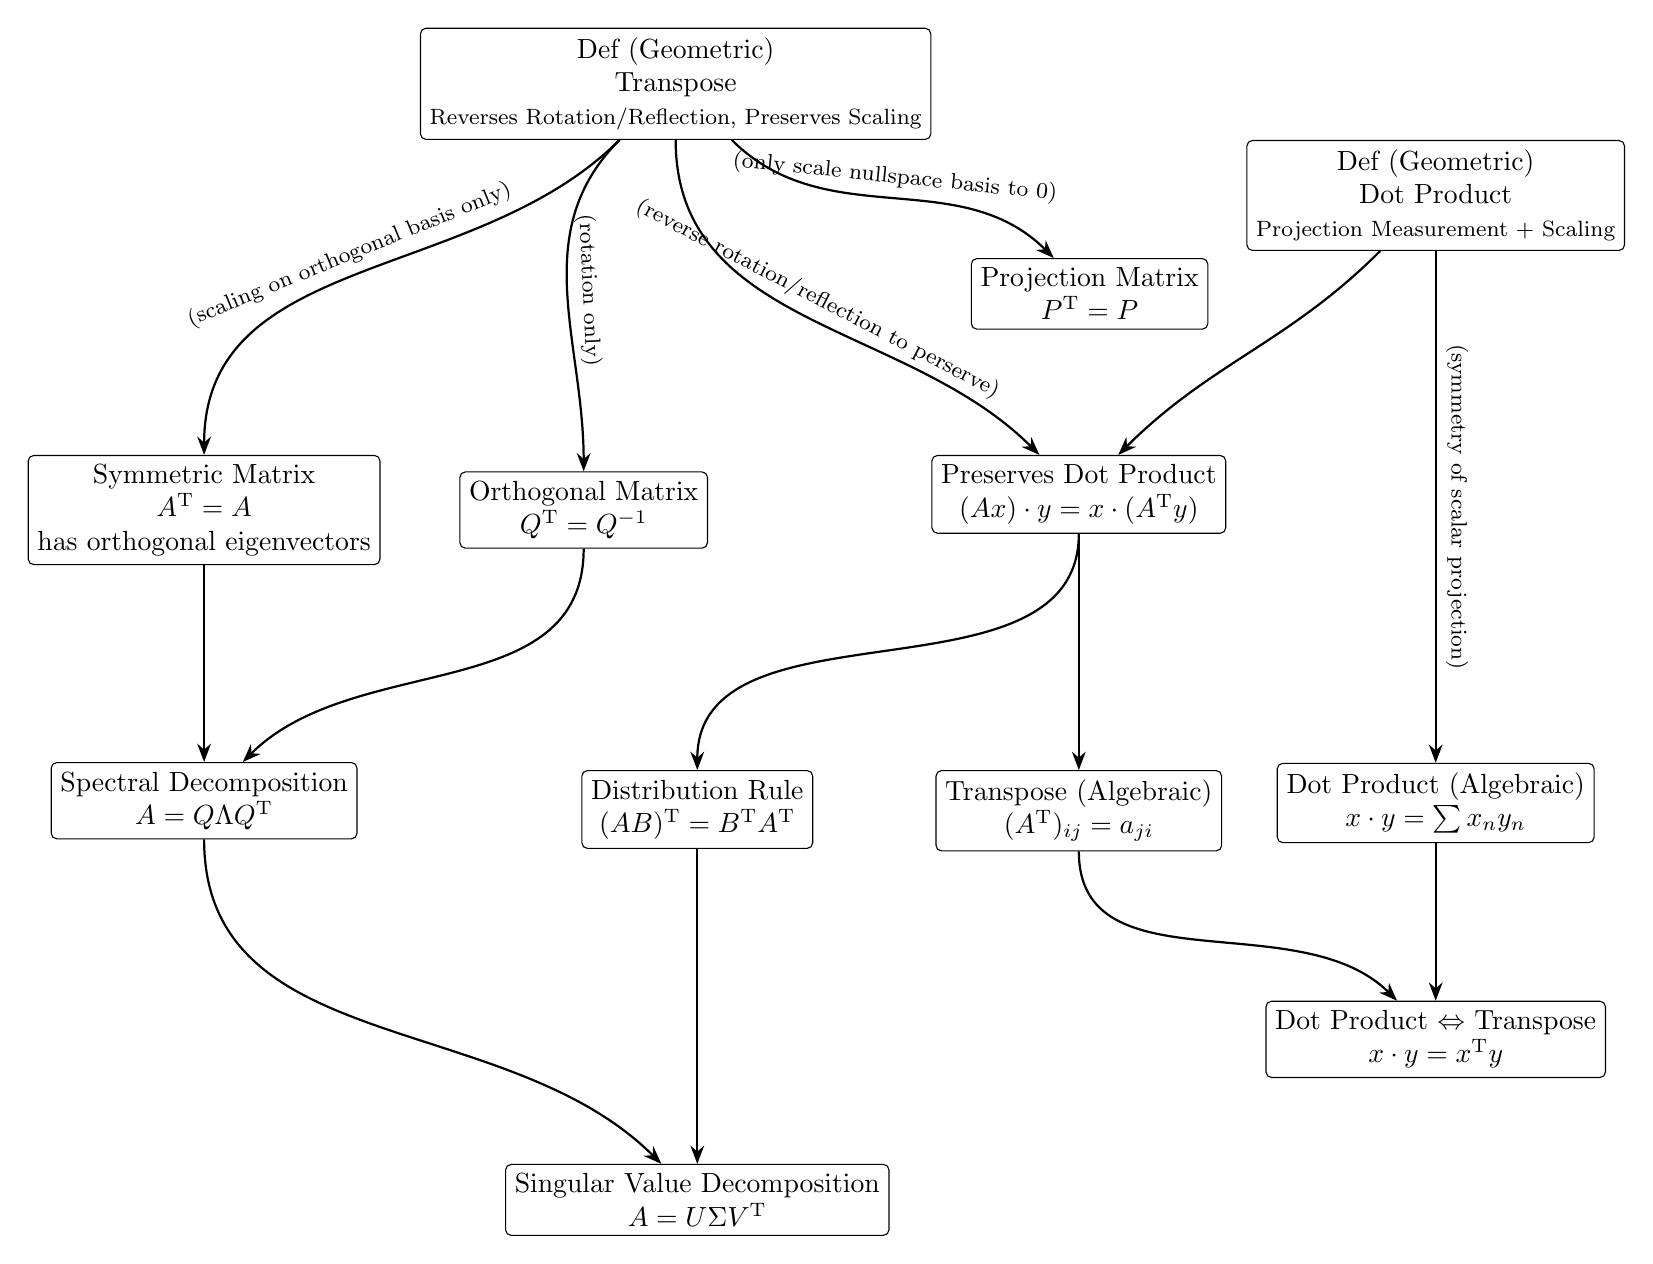
\begin{tikzpicture}[
    node distance=1.2cm and 1.5cm,
    concept/.style={align=center, draw, rounded corners=2pt},
    label/.style={sloped, font=\footnotesize, midway},
    arrow/.style={-Stealth, thick}
]
    % NODES
    \node[concept] (transpose_geo) {Def (Geometric) \\ Transpose \\ \footnotesize{Reverses Rotation/Reflection, Preserves Scaling}};
    \node[concept, below right=0cm and 4cm of transpose_geo] (dot_prod_geo) {Def (Geometric) \\ Dot Product \\ \footnotesize{Projection Measurement + Scaling}};

    \node[concept, below left=4cm and 0.5cm of transpose_geo] (symmetric) {Symmetric Matrix \\ $A^{\mathrm{T}}=A$ \\ has orthogonal eigenvectors};
    \node[concept, right=1cm of symmetric] (orthogonal) {Orthogonal Matrix \\ $Q^{\mathrm{T}}=Q^{-1}$};
    \node[concept, below right=4cm and 0cm of transpose_geo] (preserves_dot) {Preserves Dot Product \\ $(Ax) \cdot y = x \cdot (A^{\mathrm{T}} y)$};
    \node[concept, below right=1.5cm and 0.5cm of transpose_geo] (projection) {Projection Matrix \\ $P^{\mathrm{T}}=P$};

    \node[concept, below=2.5cm of symmetric] (spectral) {Spectral Decomposition \\ $A = Q \Lambda Q^{\mathrm{T}}$};
    \node[concept, below left=3cm and 1.5cm of preserves_dot] (dist_rule) {Distribution Rule \\ $(AB)^{\mathrm{T}} = B^{\mathrm{T}} A^{\mathrm{T}}$};
    \node[concept, below=3cm of preserves_dot] (transpose_alg) {Transpose (Algebraic) \\ $(A^{\mathrm{T}})_{ij} = a_{ji}$};
    \node[concept, below=6.5cm of dot_prod_geo] (dot_prod_alg) {Dot Product (Algebraic) \\ $x \cdot y = \sum x_n y_n$};

    \node[concept, below=2cm of dot_prod_alg] (dot_prod_transpose) {Dot Product $\Leftrightarrow$ Transpose \\ $x \cdot y = x^{\mathrm{T}} y$};
    \node[concept, below=4cm of dist_rule] (svd) {Singular Value Decomposition \\ $A = U \Sigma V^{\mathrm{T}}$};

    % EDGES
    \draw[arrow] (transpose_geo) to[out=-135, in=90] node[label, above] {(scaling on orthogonal basis only)} (symmetric);
    \draw[arrow] (transpose_geo) to[out=-135, in=90] node[label, above] {(rotation only)} (orthogonal);
    \draw[arrow] (transpose_geo) to[out=-90, in=135] node[label, above] {(reverse rotation/reflection to perserve)} (preserves_dot);
    \draw[arrow] (transpose_geo) to[out=-45, in=135] node[label, above] {(only scale nullspace basis to 0)} (projection);

    \draw[arrow] (symmetric) to[out=-90, in=90] (spectral);
    \draw[arrow] (orthogonal) to[out=-90, in=45] (spectral);

    \draw[arrow] (dot_prod_geo) to[out=-90, in=90] node[label, above] {(symmetry of scalar projection)} (dot_prod_alg);
    \draw[arrow] (dot_prod_geo) to[out=-135, in=45] (preserves_dot);

    \draw[arrow] (preserves_dot) to[out=-90, in=90] (transpose_alg);
    \draw[arrow] (preserves_dot) to[out=-90, in=90] (dist_rule);
    \draw[arrow] (transpose_alg) to[out=-90, in=135] (dot_prod_transpose);
    \draw[arrow] (dot_prod_alg) to[out=-90, in=90] (dot_prod_transpose);

    \draw[arrow] (spectral) to[out=-90, in=135] (svd);
    \draw[arrow] (dist_rule) to[out=-90, in=90] (svd);

\end{tikzpicture}
}
\end{figure}


\newpage
\appendix
\section{Expanded Form}

\begin{itemize}

    \item \textbf{Matrix:}
    \begin{equation}
        A =
        \left[
            \begin{array}{ccc}
                | &        & | \\
                \mathbf{a}_1 & \cdots & \mathbf{a}_n \\
                | &        & |
            \end{array}
        \right]
        \label{eq:matrix}
    \end{equation}

    \item \textbf{Inner Product:}
    \begin{equation}
        \mathbf{a}^{\mathrm{T}} \mathbf{b} =
        \left[
            \begin{array}{ccc}
                a_1 & \cdots & a_n
            \end{array}
        \right]
        \left[
            \begin{array}{c}
                b_1 \\
                \vdots \\
                b_n
            \end{array}
        \right]
        = a_1 b_1 + \cdots + a_n b_n
        \label{eq:innerprod}
    \end{equation}

    \item \textbf{Outer Product:}
    \begin{equation}
        \mathbf{a} \mathbf{b}^{\mathrm{T}} =
        \left[
            \begin{array}{c}
                a_1 \\
                \vdots \\
                a_m
            \end{array}
        \right]
        \left[
            \begin{array}{ccc}
                b_1 & \cdots & b_n
            \end{array}
        \right]
        =
        \left[
            \begin{array}{ccc}
                a_1 b_1 & \cdots & a_1 b_n \\
                \vdots & \ddots & \vdots \\
                a_m b_1 & \cdots & a_m b_n
            \end{array}
        \right]
        \label{eq:outerprod}
    \end{equation}


    \item \textbf{Matrix and Vector Multiplication - Column-wise View:}
    \begin{equation}
        A\mathbf{x} =
        \left[
            \begin{array}{ccc}
                | &        & | \\
                \mathbf{a}_1 & \cdots & \mathbf{a}_n \\
                | &        & |
            \end{array}
        \right]
        \left[
            \begin{array}{c}
                x_1 \\
                \vdots \\
                x_n
            \end{array}
        \right]
        =
        x_1\mathbf{a}_1 + x_2\mathbf{a}_2 + \cdots + x_n\mathbf{a}_n
        \label{eq:matvec_col}
    \end{equation}

    \item \textbf{Matrix and Vector Multiplication - Inner Product View:}
    \begin{equation}
        A\mathbf{x} =
        \left[
            \begin{array}{c}
                - \mathbf{a}_1^{\mathrm{T}} - \\
                \vdots \\
                - \mathbf{a}_m^{\mathrm{T}} -
            \end{array}
        \right]
        \mathbf{x}
        =
        \left[
            \begin{array}{c}
                \mathbf{a}_1^{\mathrm{T}} \mathbf{x} \\
                \vdots \\
                \mathbf{a}_m^{\mathrm{T}} \mathbf{x}
            \end{array}
        \right]
        \label{eq:matvec_row}
    \end{equation}

    \item \textbf{Row Vector and Matrix Multiplication:}
    \begin{equation}
        \mathbf{y}^{\mathrm{T}} A =
        \left[
            \begin{array}{ccc}
                y_1 & \cdots & y_m
            \end{array}
        \right]
        \left[
            \begin{array}{c}
                - \mathbf{a}_1^{\mathrm{T}} - \\
                \vdots \\
                - \mathbf{a}_m^{\mathrm{T}} -
            \end{array}
        \right]
        =
        y_1\mathbf{a}_1^{\mathrm{T}} + y_2\mathbf{a}_2^{\mathrm{T}} + \cdots + y_m\mathbf{a}_m^{\mathrm{T}}
        \label{eq:rowvecmat}
    \end{equation}

    \item \textbf{Matrix and Matrix Multiplication - Column-wise View:}
    \begin{equation}
        A B = A
        \left[
            \begin{array}{ccc}
                | &        & | \\
                \mathbf{b}_1 & \cdots & \mathbf{b}_n \\
                | &        & |
            \end{array}
        \right]
        =
        \left[
            \begin{array}{ccc}
                | &        & | \\
                A\mathbf{b}_1 & \cdots & A\mathbf{b}_n \\
                | &        & |
            \end{array}
        \right]
        \label{eq:mul_colwise}
    \end{equation}

    \item \textbf{Matrix and Matrix Multiplication - Inner Product View:}

    \begin{equation}
        AB =
        \left[
            \begin{array}{c}
                - \mathbf{a}_1^{\mathrm{T}} - \\
                \vdots \\
                - \mathbf{a}_m^{\mathrm{T}} -
            \end{array}
        \right]
        \left[
            \begin{array}{ccc}
                | &        & | \\
                \mathbf{b}_1 & \cdots & \mathbf{b}_n \\
                | &        & |
            \end{array}
        \right]
        =
        \left[
            \begin{array}{ccc}
                \mathbf{a}_1^{\mathrm{T}} \mathbf{b}_1 & \cdots & \mathbf{a}_1^{\mathrm{T}} \mathbf{b}_n \\
                \vdots & \ddots & \vdots \\
                \mathbf{a}_m^{\mathrm{T}} \mathbf{b}_1 & \cdots & \mathbf{a}_m^{\mathrm{T}} \mathbf{b}_n
            \end{array}
        \right]
        \label{eq:mul_inner}
    \end{equation}

    \item \textbf{Matrix and Matrix Multiplication - Outer Product View:}

    \begin{equation}
        AB =
        \left[
            \begin{array}{ccc}
                | &        & | \\
                \mathbf{a}_1 & \cdots & \mathbf{a}_n \\
                | &        & |
            \end{array}
        \right]
        \left[
            \begin{array}{c}
                - \mathbf{b}_1^{\mathrm{T}} - \\
                \vdots \\
                - \mathbf{b}_n^{\mathrm{T}} -
            \end{array}
        \right]
        =
        \mathbf{a}_1 \mathbf{b}_1^{\mathrm{T}} + \mathbf{a}_2 \mathbf{b}_2^{\mathrm{T}} + \cdots + \mathbf{a}_n \mathbf{b}_n^{\mathrm{T}}
        \label{eq:mul_outer}
    \end{equation}

    \item \textbf{Transpose:}
    \begin{equation}
        \left[
            \begin{array}{ccc}
                a_{11} & \cdots & a_{1n} \\
                \vdots & \ddots & \vdots \\
                a_{m1} & \cdots & a_{mn}
            \end{array}
        \right]^{\mathrm{T}}
        =
        \left[
            \begin{array}{ccc}
                a_{11} & \cdots & a_{m1} \\
                \vdots & \ddots & \vdots \\
                a_{1n} & \cdots & a_{mn}
            \end{array}
        \right]
        \label{eq:trans}
    \end{equation}

    \item \textbf{Identity Matrix:}
    \begin{equation}
        I_n =
        \left[
            \begin{array}{cccc}
                1 & 0 & \cdots & 0 \\
                0 & 1 & \cdots & 0 \\
                \vdots & \vdots & \ddots & \vdots \\
                0 & 0 & \cdots & 1
            \end{array}
        \right]
        \label{eq:iden}
    \end{equation}

    \item \textbf{Diagonal Matrix:}
    \begin{equation}
        D_n =
        \left[
            \begin{array}{cccc}
                d_1 & 0 & \cdots & 0 \\
                0 & d_2 & \cdots & 0 \\
                \vdots & \vdots & \ddots & \vdots \\
                0 & 0 & \cdots & d_n
            \end{array}
        \right]
        \label{eq:diagm}
    \end{equation}

    \item \textbf{Inverse of Diagonal Matrix:}
    \begin{equation}
        D_n^{-1} =
        \left[
            \begin{array}{cccc}
                \frac{1}{d_1} & 0 & \cdots & 0 \\
                0 & \frac{1}{d_2} & \cdots & 0 \\
                \vdots & \vdots & \ddots & \vdots \\
                0 & 0 & \cdots & \frac{1}{d_n}
            \end{array}
        \right]
        \label{eq:diagminv}
    \end{equation}

\end{itemize}

\end{document}